% !TEX root = ../Диплом.tex

\section{Полиномиализация} \label{sec:polynomialization}

\begin{definition}
    Процесс преобразования нелинейных систем \eqref{eq:ODE-norm-system}, \eqref{eq:ADE-system} к полиномиальному виду будем называть \textit{полиномиализацией}.
\end{definition}

Далее мы рассмотрим оригинальные алгоритмы квадратизации, описанные в \cite{Gu-PhD}.

\subsection{Полиномиализация с помощью введения алгебраических уравнений} \label{sec:poly-algebraic}

Следующий алгоритм проводит полиномиализацию, добавляя к системе алгебраические уравнения:
\begin{enumerate}
    \item Ввести новую переменную $y_i = g_i(\vec x)$, где $g_i(\vec x)$ - неполиномиальная нелинейная элементарная функция.
    \item Заменить $g_i(\vec x)$ на $y_i$ в оригинальном уравнении.
    \item  Добавить новое уравнение $y_i = g_i(\vec x)$ в систему.
\end{enumerate}

Показанный алгоритм приводит системы вида \eqref{eq:ODE-norm-system}, \eqref{eq:ADE-system} к полиномиальным системам вида \eqref{eq:ADE-system}

\begin{example}
    Рассмотрим уравнение $\dot x = x^3 + \frac{1}{1 + x}$. Тогда шаги алгоритма будут выглядеть следующим образом:
    \begin{enumerate}
        \item Вводим новую переменную $y = \frac{1}{1 + x}$
        \item Делаем замену в первом уравнении $\dot x = x^3 + y$
        \item  Добавляем новое уравнение в систему $y = \frac{1}{1 + x}\; \Leftrightarrow \; xy + y - 1 = 0$
    \end{enumerate}
\end{example}


Получили полиномиальную систему

$\begin{array}{lcl}
    \dot x = x^3 + y \\
    0 = xy + y - 1
\end{array}$
\newline

\begin{remark}
Важно заметить, что данный подход работает для ограниченного класса элементарных нелинейных функций, в частности для рациональных функций. Таким образом мы гарантируем полиномиальность вспомогательных уравнений. В том случае, если мы имеем дело со степенными функциями, логарифмами и многими другими элементарными нелинейностями, например $g_i(x) = e^x$, то получить полиномиальную систему данным методом мы уже не сможем.
\end{remark}


\subsection{Полиномиализация с помощью введения дифференциальных уравнений} \label{sec:poly-diff}

Второй подход к полиномиализации предлагает добавление дифференциальных уравнений к системе.
Алгоритм похож на предыдущий за исключением последнего шага:

\begin{enumerate}
    \item Ввести новую переменную $_i = g_i(\vec x)$, где $g_i(\vec x)$ - неполиномиальная нелинейная элементарная функция.
    \item Заменить $g_i(\vec x)$ на $y_i$ в оригинальном уравнении.
    \item Добавить новое уравнение $\dot y_i = \dot g_i(\vec x) = g'_i(\vec x) \dot {\vec x}$ в систему. Данное уравнение получается как сложная производная от $g_i$.
\end{enumerate}

Таким образом, мы получим систему общего вида

\begin{equation}
    \begin{array}{lcl}
        \dot x_i = p_i^T \vec x + a_{i,1} y_1 + \cdots + a_{i,m} y_m,\quad i = 1, \cdots, n \\
        \dot y_i = \pounds_{\dot{\vec x}} g_i(\vec x) = g'_i(\vec x)(p_i^T \vec x + a_{i,1} y_1 + \cdots + a_{i,m} y_m,),\quad i = 1, \cdots, m
    \end{array},
\end{equation}
\newline
где $g'(\vec x) = \frac {dg(\vec x)}{d \vec x}$, $\pounds_{\dot{\vec x}}$ - производная Ли.

Так как $g'(\vec x)$ состоит только из полиномиальных функций от $x$ и $y_i$, данная система является полиномиальной.

Данный алгоритм переводит системы к полиномиальному виду, не меняя их структуры: \eqref{eq:ODE-norm-system} $\longrightarrow$ \eqref{eq:ODE-norm-system}, \eqref{eq:ADE-system} $\longrightarrow$ \eqref{eq:ADE-system}.

\begin{example}
    Полиномиализуем уравнение $\dot x = \sin(x)$. Тогда шаги алгоритма будут выглядеть следующим образом:
    \begin{enumerate}
        \item Избавляемся от $\sin(x)$
        \begin{enumerate}
            \item Вводим новую переменную $y_1 =  \sin(x)$
            \item Делаем замену в первом уравнении $\dot x = x^3 + y$
            \item Добавляем новое уравнение в систему $\dot y_1 = \dot {\sin}(x) = \cos(x) \dot x = \sin(x) cos(x) = y_1 cos(x)$
            \item Получили систему $\begin{array}{lcl} \dot x = y_1\\ \dot y_1 = y_1 \cos(x) \end{array}$
        \end{enumerate}
        \item Избавляемся от $\cos(x)$
        \begin{enumerate}
            \item Вводим новую переменную $y_2 =  \cos(x)$
            \item Делаем замену во втором уравнении $\dot y_1 = y_1 y_2$
            \item Добавляем новое уравнение в систему $\dot y_2 = \dot {\cos}(x) = -\sin(x) \dot x = -y_1^2$
        \end{enumerate}
    \end{enumerate}
    
    Получили полиномиальную систему
    
    $\begin{array}{lcl}
        \dot x = y_1\\
        \dot y_1 = y_1 y_2\\
        \dot y_2 = -y_1^2
    \end{array}$
\end{example}



\begin{theorem} \label{theorem:polynomialization}
    \begin{enumerate}
    \item Итеративно применяя алгоритмы полиномиализации с помощью введения алгебраических и дифференциальных уравнений, нелинейную систему с элементарными нелинейностями можно привести к полиномиальной форме.
    \item Размер полученной полиномиальной системы является линейным относительно числа элементарных функций в     оригинальной системе.
\end{enumerate}
\end{theorem}

\begin{proof}
    Доказательство первой части теоремы уже изложено вместе с алгоритмами полиномиализации.
    
    Рассмотрим вторую часть.
    Заметим, что для того, чтобы избавиться от основной (не композитной) элементарной функции,
    требуется конечное число замен $O(1)$, обычно 1 или 2, например для $sin(x)$.
    
    Для композитных элементарных функций $g(\vec x) = (g_1 \circ g_2 ... \circ g_n)(\vec x)$ необходимо потратить $O(1 \cdot m)$ замен.
    Таким образом, размер полученной полиномиальной системы линеен относительно числа элементарных функций в оригинальной системе.
\end{proof}

\subsection{Анализ оригинальных алгоритмов}

Мы показали, что с помощью оригинальных алгоритмов всегда можно провести полиномиализацию, однако провести её можно разными способами, вводя при этом разное количество переменных \cite{Gu-PhD}. Тем не менее, из теоремы \ref{theorem:polynomialization} мы знаем, что максимальное число введённых переменных всегда линейно от относительно числа элементарных функций в оригинальной системе. Таким образом, мы можем сосредоточится на скорости алгоритма полиномиализации, оставляя при этом возможность получать достаточно оптимальные преобразования.

\subsection{Абстрактные синтаксические деревья} \label{sec:AST}

Для того, чтобы удобно работать с математическими выражениями, нам понадобится определить на них структуру.
Для этого мы воспользуемся синтаксическим анализом - процессом преобразования последовательности лексем формального языка с его формальной грамматикой.
Результатом обычно является дерево разбора, которое отражает синтаксическую структуру входной последовательности лексем.

\begin{figure}[h!]
    \centering
    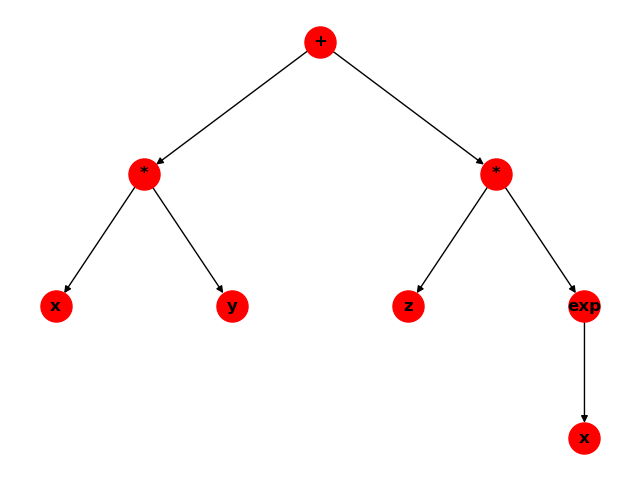
\includegraphics{chapters/images/AST.png}
    \caption{Абстрактное синтаксическое дерево выражения $x \cdot y + z \cdot exp(x)$}
    \label{fig:AST}
\end{figure}

В нашем случае мы получаем на вход строковое представление математического выражения, а возвращаем дерево разбора, состоящее из внутренних узлов, представляющий математические функции, например как сложение или взятие логарифма, и листьев, состоящих из переменных и чисел.

Абстрактное синтаксическое дерево (\textit{АСД}, \textit{AST}) отличается от дерева разбора тем, что в нём отсутствуют узла и рёбра, которые не влияют на семантические свойств выражения. Например, для выражения $3 + 2 \cdot 4$ не нужно расставлять группирующие скобки, так как приоритет операции умножения задан выше, чем приоритет операции сложения.

Многие языки программирования и системы компьютерной алгебры используют данный подход для обработки для обработки своих выражений. В частности, АСД использует фреймворк SymPy \cite{SymPy}, реализованный на языках программирования Python и Julia, который мы будем использовать в дальнейшем.

Подробнее ознакомиться с синтаксическими деревьями можно в \cite{Automata-book}, \cite{Compilers-book}

\subsection{Алгоритм полиномиализации} \label{poly-algo}

Для начала перепишем алгоритмы из секций \ref{sec:poly-algebraic}, \ref{sec:poly-diff} в формальном общем виде. Как уже упоминалось в разделе \ref{sec:AST}, нам удобно представлять правые части уравнений системы в виде абстрактных синтаксических деревьев. Из таких деревьев мы формируем лес, которые впоследствии мы будем анализировать.

\begin{algorithm}[H]
\SetAlgoLined
\SetKwFunction{FPoly}{Polynomialize}
\SetKwFunction{FGetNonPoly}{GetNonPolynomialItem}
\SetKwFunction{FFindNonPoly}{FindNonPolynomialItem}
\SetKwProg{Fn}{Function}{:}{}
\KwData{System - система вида \eqref{eq:ODE-norm-system} или \eqref{eq:ADE-system}}
\KwResult{Полиномиализированная система}
\Fn{\FPoly{System}}{
    NewSystem = Копия(System)\;
    
    \tcc{Лес абстрактных синтаксических деревьев}
    Forest = \{\quad\}\;
    
    \tcc{массив меток, где true - данное дерево не содержит неполиномиальных элементов}
    ForestIsPoly = \{\quad\}\;
    
    \ForEach{r: правое уравнение системы}{
        tree = AST(r)\;
        Добавить(Forest, tree)\;
        ForestIsPoly[tree] = false\;
    }
    
    \While{ForestIsPoly содержит false}{
        g = \FGetNonPoly{Forest, ForestIsPoly}\;
        ДобавитьУравнение(NewSystem, g)\;
    }
    
    \Return NewSystem\;
}
\BlankLine
\BlankLine
\Fn{\FGetNonPoly{Forest, ForestIsPoly}}{
    \ForEach{tree: ForestIsPoly[tree] == false}{
        nonPolyItem = \FFindNonPoly{tree}\;
        \eIf{nonPolyItem $\ne$ null }{
            \Return nonPolyItem\;
        }{
            ForestIsPoly[tree] = true\;
        }
    }
    \Return null\;
}
\caption{Полиномиализация}
\end{algorithm}

\subsubsection{Прямой обход}

Разберём вариант реализации алгоритма FindNonPolynomialItem, который предполагает прямой проход по синтаксическому дереву - от корня к листьям. \\

\begin{algorithm}[H]
\SetAlgoLined
\SetKwFunction{FFindNonPoly}{FindNonPolynomialItem}
\SetKwProg{Fn}{Function}{:}{}
\KwData{node - узел AST, составленного из правой части уравнения системы \eqref{eq:ODE-norm-system} или \eqref{eq:ADE-system}}
\KwResult{Неполиномиальный элемент или null, если такой не найдётся}

\Fn{\FFindNonPoly{node}}{
    \If{неПолиномиальнаяФункция(node)}{
        \Return node\;
    }
    
    \ForEach{child: дети node}{
        nonPolyItem = \FFindNonPoly{child}\;
        \If{nonPolyItem $\ne$ null}{
            \Return nonPolyItem\;
        }
    }
    \Return null\;
}

\caption{Прямой обход синтаксического дерева}
\end{algorithm}

\newpage

\subsubsection{Обратный обход}

Теперь рассмотрим вариант реализации алгоритма FindNonPolynomialItem, который предполагает обратный проход по синтаксическому дереву - от листьев к корню. \\

\begin{algorithm}[H]
\SetAlgoLined
\SetKwFunction{FFindNonPoly}{FindNonPolynomialItem}
\SetKwProg{Fn}{Function}{:}{}
\KwData{node - узел AST, составленного из правой части уравнения системы \eqref{eq:ODE-norm-system} или \eqref{eq:ADE-system}}
\KwResult{Неполиномиальный элемент или null, если такой не найдётся}

\Fn{\FFindNonPoly{node}}{
    \ForEach{child: дети node}{
        nonPolyItem = \FFindNonPoly{child}\;
        \If{nonPolyItem $\ne$ null}{
            \Return nonPolyItem\;
        }
    }
    
    \If{неПолиномиальнаяФункция(node)}{
        \Return node\;
    }
    \Return null\;
}

\caption{Обратный обход синтаксического дерева}
\end{algorithm}

\subsubsection{Сравнение}

Прямой и обратный обходы по синтаксическому дереву похожи на поиск в ширину и поиск в глубину соответственно. \\

Прямой обход последовательно проходит уровни глубины синтаксического дерева, возвращая первый встреченный неполиномиальный элемент. Таким образом, данный алгоритм работает быстрее, чем обратный подход в том случае, когда  нелинейный элемент находится неглубоко, что характерно для для практических задач. Однако важно помнить, что если найденный нелинейный элемент является композицией функций $g = g_1 \circ g_2 \circ \cdots \circ g_k$, то прямой обход вернёт всю композицию. Это является существенным недостатком, если мы используем алгоритм \ref{sec:poly-diff}, требующий вычислять сложную производную функции $g$, что является весьма дорогой операцией для композиции функций.

Обратный обход, в свою очередь, ищет самые глубоко вложенные неполиномиальные элементы $g_k$. Поэтому, он всегда находит базовые элементарные функции, имеющие тривиальные производные, затрачивая, в целом, большее число шагов.    

\begin{example}
    Для выражения $x + \sin{(\exp{x})}$ прямой обход найдёт найдёт $\sin{(\exp{x})}$, а обратный - $\exp{x}$.
\end{example}

Таким образом, для полиномиализации \ref{sec:poly-algebraic} мы предпочтём прямой обход, а для \ref{sec:poly-diff} - обратный.
